\section{Risk factors of stablecoins}\label{sec:risk_factors}

The holding leg of the stablecoin workflow is where the expected loss lives. A holder of a fiat-backed stablecoin carries, however briefly, a private-issuer liability convertible into the fiat unit of account at par on a best-effort basis. That promise can fail in two ways, and the two failures are economically distinct. The issuer may not hold enough liquid reserves of sufficient credit quality to honour redemption at par, in which case the holder bears a \emph{counterparty} loss. Or the market for converting the liability outside the issuer's primary venue may be too thin, so the realised conversion price falls below par when demand to convert is high, in which case the holder bears a \emph{depeg} loss. The holding leg therefore carries an expected loss with two components. This section sets out each in turn: a counterparty component, an issuer-level credit exposure we read from market proxies; and a depeg component, whose baseline piece is the observable cost of converting under normal conditions and whose stress piece is a coordination outcome we price with the closed-form global game of Section~\ref{sec:model}. Figure~\ref{fig:workflows} places both alongside the traditional workflow, locating where each cost lives and where the model is needed.

\begin{figure}[t]
\centering
\begin{tikzpicture}[
  font=\footnotesize, >=Latex,
  box/.style={draw, rounded corners=2pt, minimum width=2.0cm, minimum height=8mm, inner sep=3pt, align=center},
  trad/.style={box, fill=blue!8},
  stab/.style={box, fill=red!7},
  hold/.style={box, fill=green!12, minimum width=2.4cm, minimum height=10mm, very thick},
  cost/.style={font=\scriptsize\itshape, align=center, text=black!70},
  note/.style={font=\scriptsize, align=center}
]
% ===== Panel (a): traditional rail =====
\node[note, anchor=west, font=\footnotesize\bfseries] (htA) at (0,3.4) {(a) Traditional rail (RTGS / SWIFT)};
\node[trad] (ta) at (1.4,2.5) {sender};
\node[trad, right=1.7cm of ta] (tb) {bank rail\\(RTGS/SWIFT)};
\node[trad, right=1.7cm of tb] (tc) {recipient};
\draw[->] (ta) -- node[cost, above]{fee + FX} (tb);
\draw[->] (tb) -- node[cost, above]{} (tc);
\node[note, below=1.5mm of tb, text=blue!45!black, text width=5.2cm] {asset held $=$ bank deposit,\\ backed by a supervised, insured bank};
\node[note, right=1.2cm of tc, text width=2.6cm, font=\footnotesize\bfseries, text=blue!45!black] {expected loss\\ on the asset $= 0$};
% ===== Panel (b): stablecoin circuit =====
\node[note, anchor=west, font=\footnotesize\bfseries] (htB) at (0,1.0) {(b) Stablecoin circuit (fiat to fiat)};
\node[stab] (sa) at (1.1,0.0) {fiat};
\node[stab, right=1.0cm of sa] (sb) {on-ramp};
\node[hold, right=1.0cm of sb] (sc) {hold coin};
\node[stab, right=1.0cm of sc] (sd) {off-ramp};
\node[stab, right=1.0cm of sd] (se) {local fiat};
\draw[->] (sa) -- (sb);
\draw[->] (sb) -- node[cost, above]{on-chain fee} (sc);
\draw[->] (sc) -- (sd);
\draw[->] (sd) -- (se);
% cost labels BELOW each leg, on one clean row, no overlap
\node[cost, below=1.5mm of sb, text=red!55!black] {platform fee\\(observable)};
\node[cost, below=1.5mm of sd, text=red!55!black] {basis $+$ fee\\(observable)};
\node[note, below=1.5mm of sc, text width=3.0cm, text=green!35!black] {$\ell_C$ counterparty (obs.)\\$+\;p_s\times$ stress depeg};
% the global game annotation, clearly attached to the holding leg
\node[draw, rounded corners=2pt, fill=green!6, font=\scriptsize, align=center, text=green!35!black,
      below=1.4cm of sc, text width=3.4cm] (gg) {\textbf{stress depeg} priced by the\\ closed-form \textbf{global game}\\ (run probability $p_s$)};
\draw[->, green!45!black, dashed] (gg) -- (sc);
\end{tikzpicture}
\caption{Two payment workflows. On the traditional rail (a) the asset the payer briefly holds is a bank deposit, backed by a supervised and insured bank, so its expected loss is zero. On the stablecoin circuit (b) the payer runs fiat to fiat through five legs: the on-ramp and off-ramp platform fees and the on-chain fee are observable, the off-ramp also carries the conversion basis, and the holding leg carries the expected loss, the observable counterparty exposure $\ell_C$ plus the stress depeg, the one piece priced by the closed-form global game through its run probability $p_s$.}\label{fig:workflows}
\end{figure}

\subsection{Counterparty credit risk}\label{sub:counterparty}

The counterparty component is the expected loss from issuer default. A holder of one unit faces an annualised default hazard $h$ and, conditional on default, a loss given default $\xi$ equal to the shortfall of recoverable reserve value against par, so the expected per-unit loss over an exposure window of $T$ years is $h \cdot T \cdot \xi$. This is a standard credit exposure on a short-dated claim against a private issuer; it does not depend on the redemption behaviour of other holders, and we price it in reduced form from observable proxies rather than from the coordination model of the next subsection.

The window $T$ requires a choice that comparisons of stablecoin costs usually leave implicit. The exposure of a payment is not the seconds the transfer spends on chain: it runs from the sender's on-ramp to the recipient's off-ramp, and on the corridors we price the representative holder does not off-ramp on arrival. Retail stablecoin balances on Latin American corridors double as a dollar store of value between transfers, and a recurrent sender or a receiving merchant maintains a standing working balance \citep{chainalysis_2025, aldasoro_frost_ito_2026}. We price that continuous-balance holder and set $T = 1$, so the counterparty component reads as the annual carrying cost of the working balance the payment chain maintains, and we write $\ell_C = h \xi$ with $T$ suppressed hereafter. The polar opposite case bounds what the choice contributes: a transit-only payment that off-ramps within a day carries a counterparty loss of $h\xi/365$, a fraction of a basis point for either coin, and for such a user the expected loss reduces to the depeg block alone, 29.0 basis points for USDC and 11.2 for USDT in the decomposition of Section~\ref{sec:identification}. The headline expected loss is therefore the cost borne by the holder whose balances make the corridor function, not a charge mechanically attached to every transit.

The proxies that discipline $h$ and $\xi$ exist for both issuers, and they point in different directions. USDC is backed exclusively by short-dated US Treasuries and cash deposits at globally systemic banks, with monthly attestations and daily disclosure of holdings since 2022; its reserve is transparent and its loss given default correspondingly low. USDT holds a heterogeneous mix of US Treasuries, secured loans, and historically commercial paper, with attestations produced by BDO that lack the granularity of a full audit, and a residual uncertainty compounded by its enforcement record (the 2021 New York Attorney General and CFTC settlements). The implication for the model is direct: USDC's loss-given-default parameter $\xi$ is structurally lower than USDT's, and USDT's hazard $h$ is structurally higher. On the counterparty dimension the two coins are different animals, and a single number applied to both would misprice one of them.

Three observable magnitudes discipline the central values, so that $(h, \xi)$ are anchored rather than assumed. First, attested reserve composition disciplines $\xi$. Circle publishes monthly third-party attestations and daily holdings disclosure of a reserve held in short-dated US Treasuries and cash at systemically supervised banks, so the recoverable value in a default is high and $\xi = 0.20$ is a conservative haircut on the least liquid slice; Tether's attestations, produced by BDO at a quarterly cadence without full-audit granularity, leave a material share of the reserve in secured loans and other non-Treasury assets, supporting the higher $\xi = 0.30$. Second, the enforcement record disciplines the ordering and rough level of $h$. The 2021 New York Attorney General and CFTC settlements documented that Tether's reserve backing had been incomplete for extended periods,\footnote{The CFTC order of October 2021 found that Tether held sufficient fiat reserves to back the outstanding supply on only about a quarter of the days in a 26-month sample over 2016--2018.} a disclosure history with no USDC counterpart, and one-year hazards of one and two percent correspond to the historical default experience of speculative-grade issuers in the BB-to-B band \citep{sp_default_study_2025}, the standing we judge consistent with private financial issuers operating without access to resolution backstops, with the one-notch gap reflecting that record. Third, the market's own stress pricing bounds the product $h\xi$ from above: the deepest secondary discounts recorded for the two coins, roughly 500 basis points for USDT in October 2018 \citep{lyons_viswanath_natraj_2023} and 980 for USDC in March 2023, are conditional-on-stress readings of the market's expected loss, and an unconditional annual expected loss of 20 to 60 basis points sits an order of magnitude below those conditional readings, as it must if stress regimes are rare. The Merton-style equity-to-hazard mapping introduced for the regulatory band in Appendix~\ref{app:sensitivity} ties $h$ to a market observable for the listed issuer: the same elasticity that converts an adverse equity correction into a hazard rise reads in reverse as a check that the central level is not understated in calm conditions.

We set $h=0.01$ and $\xi=0.20$ for USDC and $h=0.02$ and $\xi=0.30$ for USDT at the centre of these anchors. The product $h\,\xi$ is the \emph{expected}, not the stressed, counterparty loss: the ten-cent intraday discount USDC reached during the March 2023 banking weekend is a depeg, priced by the global game below, not a realised default, and the resulting counterparty component of twenty basis points is the small ex-ante hazard rather than that ex-post discount. The internet appendix reports how the expected loss moves as $(h,\xi)$ range over their plausible values, and Appendix~\ref{app:sensitivity} the episode-conditional regulatory band.

\subsection{Depeg risk and the global game}\label{sub:depeg}\label{sec:global_game_policy}

The depeg component is not a credit exposure but a coordination outcome. Even a fully solvent issuer can deliver below par when many holders convert at once: primary redemption pays par only up to liquid reserves $R$, unmet demand spills into a secondary market of finite, stress-contracting depth, and the realised conversion price falls. A holder who anticipates others converting at the same time anticipates a worse price, so the decision is strategic, not individual. We model it as a global game in the spirit of \citet{morris_shin_1998}, adapted to the dual-channel exit through the issuer's primary redemption and a secondary market with depth-dependent price impact that distinguishes a stablecoin from a deposit. Figure~\ref{fig:global_game} shows the coordination structure.

\begin{figure}[p]
\centering
\includegraphics[width=\textwidth]{figures/fig_morris_shin_clock_preview.pdf}
\caption{The two risk components and their pricing routes. The counterparty loss does not depend on other holders' behaviour, so it is priced in reduced form from market observables (left route): attested reserve composition disciplines $\xi$ and the enforcement record disciplines $h$. The depeg loss is an equilibrium outcome, priced by the global game (right route): regime priors disciplined by the hourly price data and private signals determine a unique redemption threshold, whose conversion mass moves the secondary price. The two components combine additively into the expected loss $\Pi_{\text{risk}}$. The formal model is in Section~\ref{sec:model}.}\label{fig:global_game}
\end{figure}

A global game is the natural model rather than a stylised analogy because the secondary conversion price is not a market prior but an equilibrium object: the value of converting depends on how many others convert, through the price impact their conversions create, so the redemption decision is a coordination problem with a unique threshold equilibrium. That uniqueness is what lets the calibration map an observed price path into a single expected loss. The depth and convexity of the secondary market are themselves structural primitives that differ across issuers: USDT is the most liquid stablecoin globally, with primary venue Binance and per-side depth above USD 100 million, so its price-impact scale and depth erosion are structurally smaller, whereas USDC's venue (Coinbase) is shallower and its permissionless redemption more atomistic, raising its signal noise.

The two largest historical depeg episodes show the phenomenon directly, and they are the episodes we calibrate to. Figure~\ref{fig:svb_onchain} plots USDC during the March 2023 Silicon Valley Bank failure: the secondary price fell to about 0.90, the shaded below-par area being the holder's loss, as Circle's primary redemption was constrained by the banking closure; the on-chain redemptions that clear at par surged only once the federal backstop restored the peg. Figure~\ref{fig:terra_onchain} is the mirror image, USDT during the May 2022 Terra collapse: primary redemption stayed open, about USD 8 billion was redeemed at par, and the depeg was a brief dip to 0.975. The depth of a depeg thus turns on whether primary redemption remains available, the mechanism the global game formalises and Section~\ref{sec:identification} tests.

\begin{figure}[H]
\centering
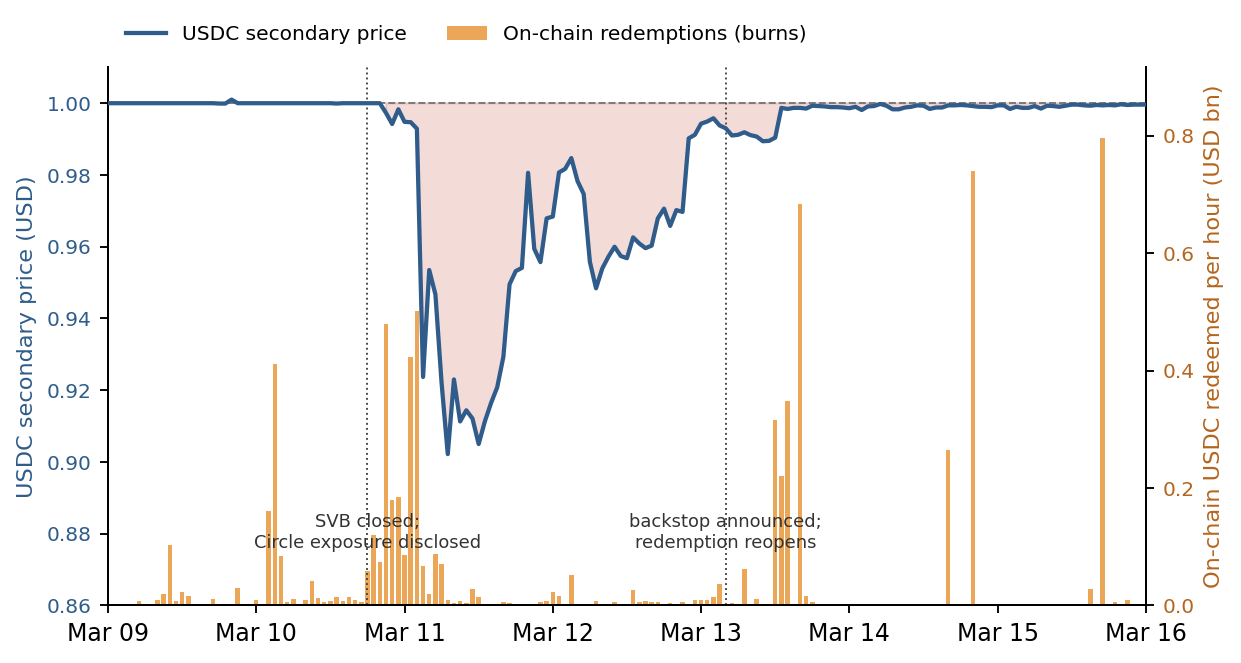
\includegraphics[width=\textwidth]{figures/fig_svb_onchain.pdf}
\caption{USDC during the March 2023 Silicon Valley Bank episode. Left axis: the hourly USDC secondary price, with the shaded area marking the below-par depeg. Right axis: hourly on-chain redemptions (token burns), from Etherscan. The depeg opens while primary redemption is constrained by the banking closure over 11--12 March; the at-par on-chain redemptions are largest only after the federal backstop restores the peg on 13 March. The holder's cost is the secondary discount borne while par redemption is unavailable, not the orderly redemptions that follow.}\label{fig:svb_onchain}
\end{figure}

\begin{figure}[H]
\centering
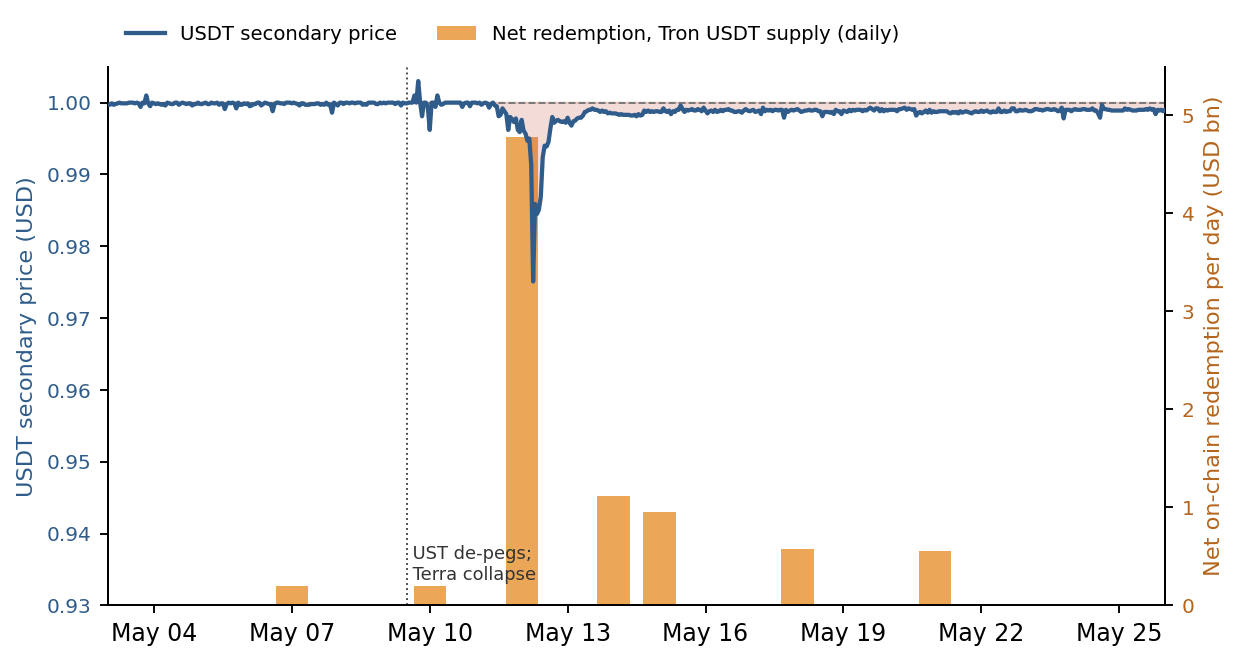
\includegraphics[width=\textwidth]{figures/fig_terra_onchain.pdf}
\caption{USDT during the May 2022 Terra episode. Left axis: the hourly USDT secondary price, with the below-par depeg shaded. Right axis: daily net redemption, measured as the contraction of USDT's Tron circulating supply. Primary redemption stayed open, about USD 8 billion was redeemed at par, and the depeg was a brief dip to 0.975, the mirror image of the USDC episode in Figure~\ref{fig:svb_onchain}.}\label{fig:terra_onchain}
\end{figure}

Section~\ref{sec:model} sets out the model formally, and Section~\ref{sub:what_it_delivers} combines the two risks into the expected loss the holder bears.
